\ffigbox[\FBwidth]{%
\caption{\centering Graphe \(G'\) simplifié}\label{fig:dm1_ex01_f6}
}{
    \fbox{
        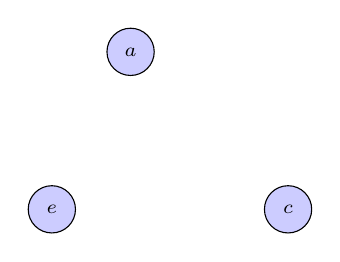
\begin{tikzpicture}[scale=1, main node/.style={circle, draw, fill=blue!20, inner sep=1pt, font=\scriptsize, minimum size=6mm, text=black}]
            % les sommets initiaux
            \node[main node] (a) at (0,0) {\(a\)};
            \node[main node] (c) at (2,-2) {\(c\)};
            \node[main node] (e) at (-1,-2) {\(e\)};
        \end{tikzpicture}
    }
}